\NeedsTeXFormat{LaTeX2e}
\documentclass[12pt,oneside,a4paper]{article}
\usepackage[left=2cm, right=2cm, top=1cm, bottom=2cm]{geometry}
\usepackage{amsmath,amsfonts,amssymb,amsthm}
\usepackage[utf8]{vietnam}
\usepackage{graphicx}
\usepackage[american]{circuitikz}
\usepackage{float}
\usepackage{mathptmx}
\usepackage{multicol}
\usepackage{enumitem} 
\usepackage{tasks} 
\usepackage{booktabs}
\usepackage{array}
\usepackage{caption}
\usepackage{hyperref}

\everymath{\displaystyle}
\theoremstyle{definition}
\newtheorem{bt}{} 
\renewcommand{\thebt}{\textbf{\large Q\arabic{bt}}} 

\newcommand{\bb}[1]{\mathbb{#1}}

\newlist{questions}{enumerate}{1}
\setlist[questions]{label=\textbf{Q$_{\mathbf{\arabic*}}$:}, leftmargin=4em}

\settasks{label=\textbf{\Alph*.}, label-width=1.5em, item-indent=7mm}

\begin{document}
	\renewcommand{\figurename}{Figure}
	\renewcommand{\tablename}{Table}
	
	\begin{center}
		\textbf{\Large EXPERIMENT 5}
		
		\vspace{0.5cm}
		\textbf{{\Large INVESTIGATION OF TRANSMISSION OF}}
		
		\vspace{0.1cm}
		\textbf{{\Large ELECTROMAGNETIC WAVE (MICROWAVE)}}
	\end{center}
	
	\vspace{0.5cm}
	
	\noindent
	\begin{minipage}[t]{0.5\textwidth}
		\vspace{0.5cm}
		\textbf{Class: IT-E10 02} \\[0.2cm]
		\textbf{Group: 3} \\[0.2cm]
		\textbf{Name: Nguyễn Trọng Phúc Anh} \\[0.2cm]
		\textbf{Student ID: 202516522}
	\end{minipage}%
	\begin{minipage}[t]{0.5\textwidth}
		\vspace{0pt}
		\centering
		\textit{\textbf{Verification of the instructors}} \\[0.2cm]
		\begin{tabular}{|p{3.5cm}|p{3.5cm}|}
			\hline
			& \\[2.5cm]
			\hline
		\end{tabular}
	\end{minipage}
	
	\vspace{0.8cm}
	
	\section*{1. THEORETICAL BACKGROUND}
	Microwaves are radio waves belonging to the electromagnetic (EM) spectrum whose wavelengths are conveniently measured in a few centimeters, corresponding to frequencies ranging from roughly $1.0\text{ GHz}$ to $30\text{ GHz}$. The small wavelength of microwaves allows conveniently sized antennas to direct them in narrow beams, which can be pointed directly at the receiving antenna.
	
	\vspace{0.3cm}
	\noindent
	Microwave radio transmission is commonly used:
	\begin{itemize}[leftmargin=1.5em]
		\item In point-to-point communication systems on the surface of the Earth, in satellite communications, and in deep-space radio communications.
		\item For radars, radio navigation systems, sensor systems, and radio astronomy.
	\end{itemize}
	
	\vspace{0.2cm}
	\noindent
	The components and equipment included allow various experiments to be performed. A narrow beam of electromagnetic waves with a wavelength in the centimeter range (microwaves) in the form of a square-modulated signal is generated by the control unit, output by a transmitter, and picked up using accessories such as a horn antenna or a sensor probe. The modulation of the received signal can be rendered audible by means of an internal speaker, and the intensity of the signal can also be controlled.
	
	\section*{2. EXPERIMENTAL PROCEDURE}
	\subsection*{2.1. Straight-line propagation of microwaves}
	\begin{center}
		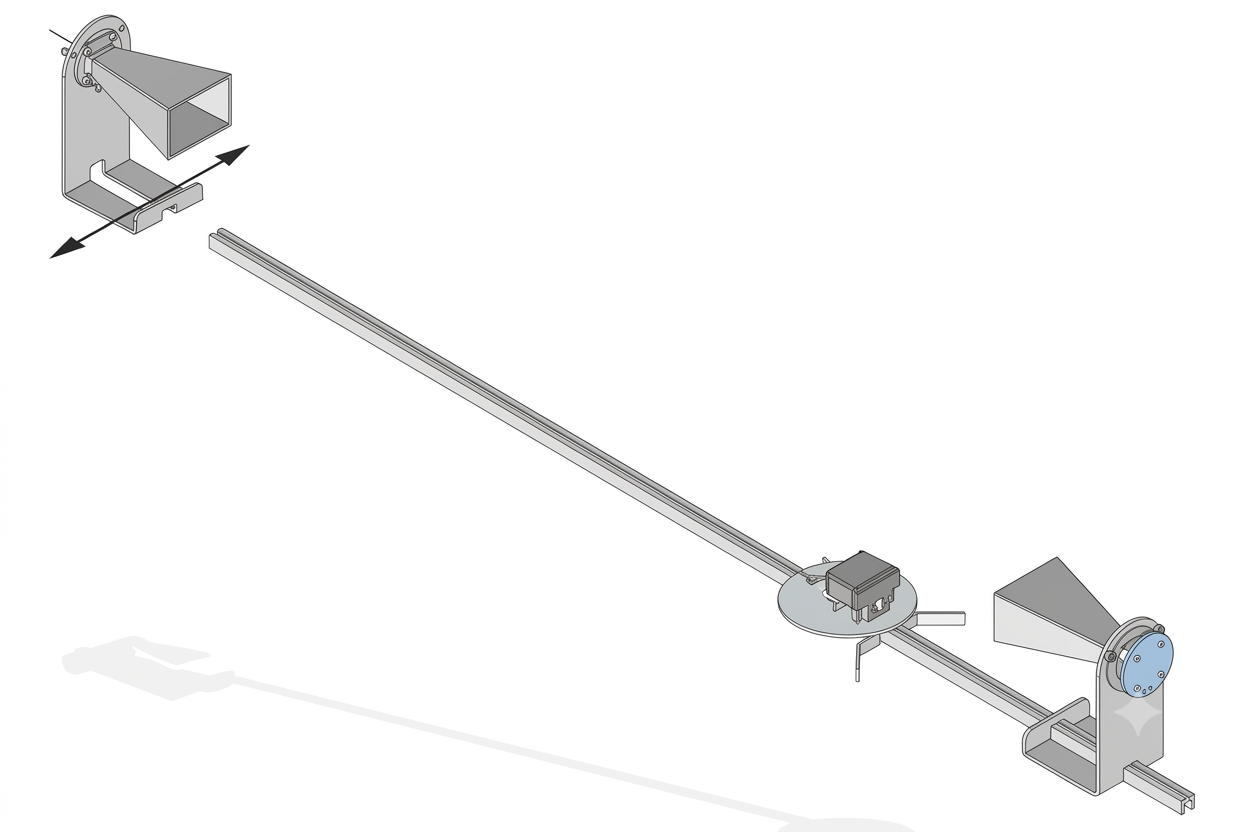
\includegraphics[width=0.5\textwidth]{Fig1}
		\captionof{figure}{\textit{Experimental setup for straight-line propagation of microwaves}}
	\end{center}
	\begin{enumerate}[leftmargin=1.5em]
		\item Set up the transmitter and receiver facing one another with the receiver off the rail, as shown in Fig. 1.
		\item Move the receiver in a plane perpendicular to the rail. Observe and draw a conclusion on the optimum position of the horns for reception.
	\end{enumerate}
	
	\subsection*{2.2. Penetration of microwaves}
	\begin{center}
		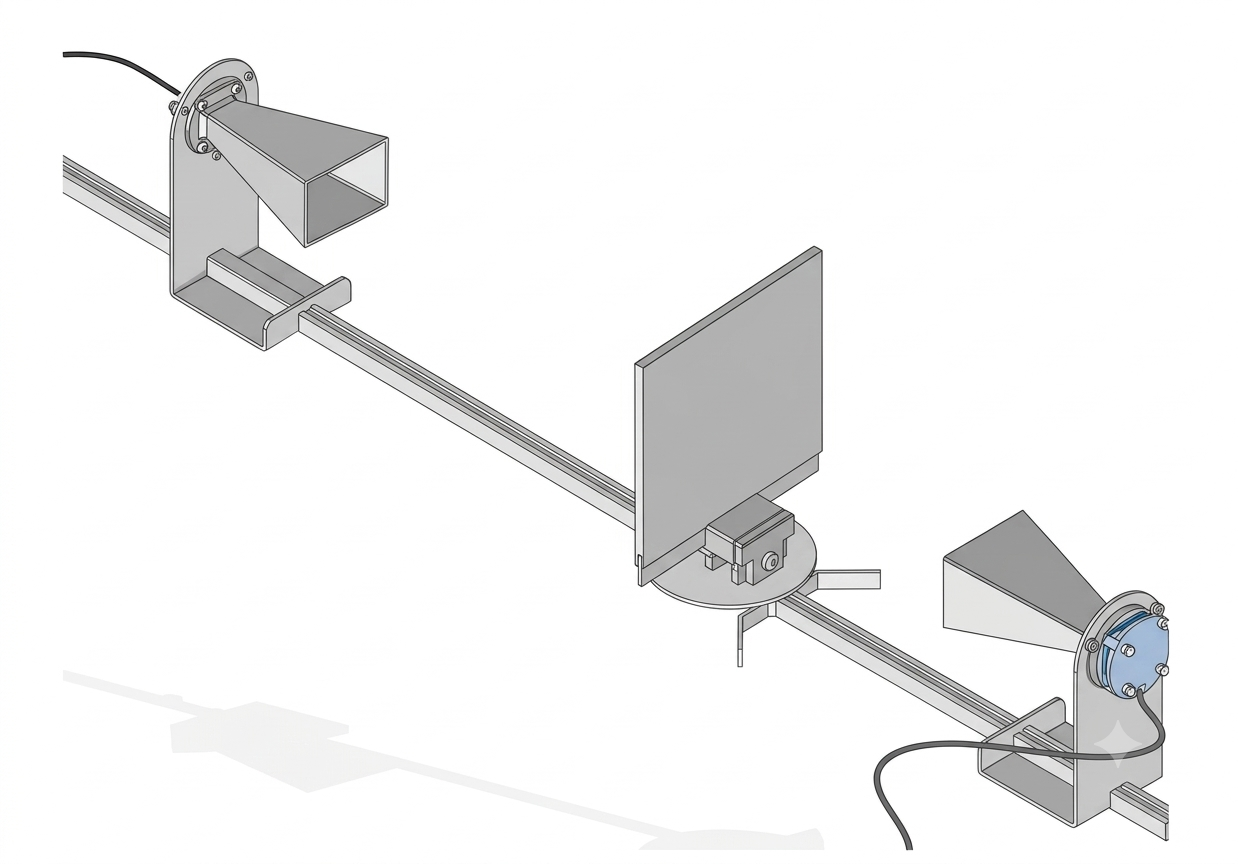
\includegraphics[width=0.5\textwidth]{Fig2}
		\captionof{figure}{\textit{Experimental setup for penetration of microwaves}}
	\end{center}
	\begin{enumerate}[leftmargin=1.5em]
		\item Set up the transmitter and receiver facing one another.
		\item Attach the dry absorption plate (electrical insulator) to the plate holder and place it between the transmitter and receiver, as shown in Fig. 2.
		\item Set the amplification to a medium level. Observe and draw a conclusion on the reception of the signal.
	\end{enumerate}
	
	\subsection*{2.3. Screening and absorption of microwaves}
	\begin{center}
		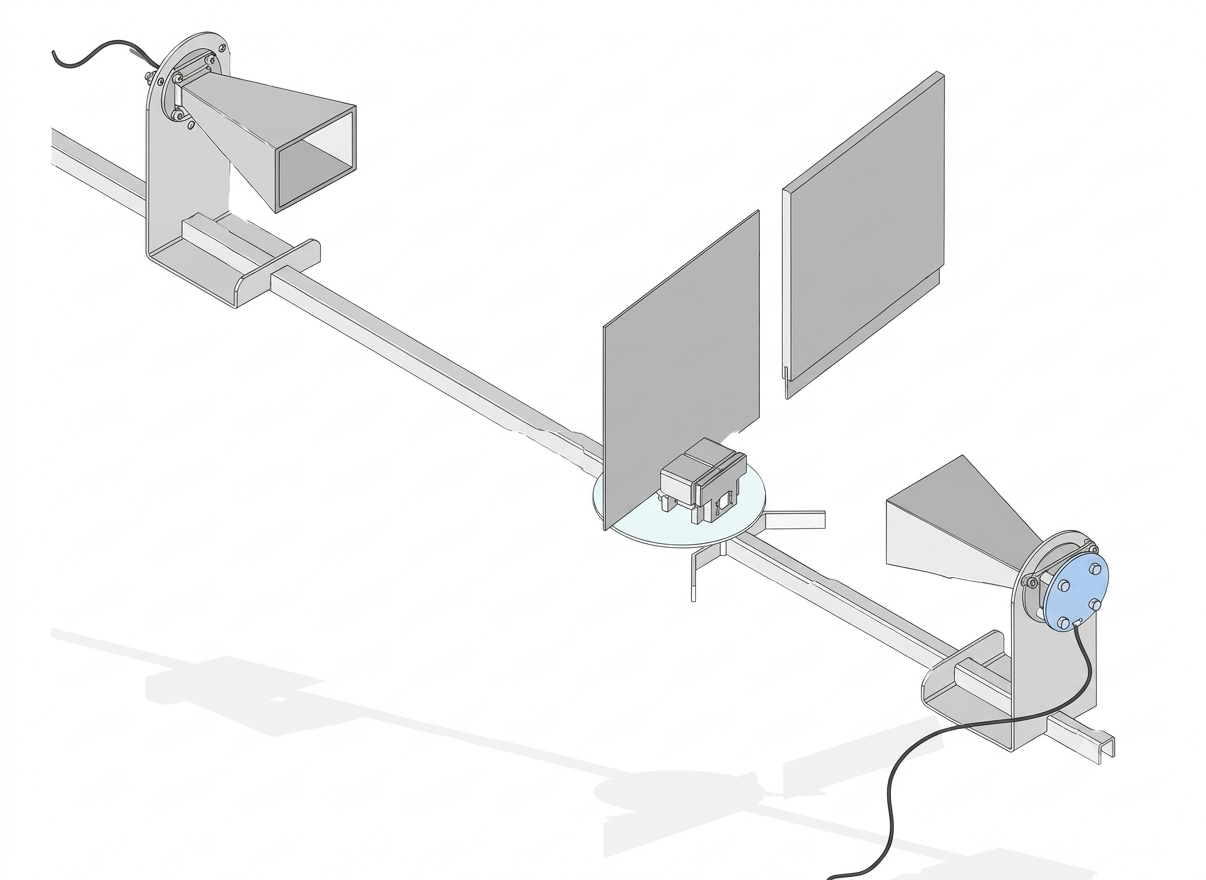
\includegraphics[width=0.5\textwidth]{Fig3}
		\captionof{figure}{\textit{Experimental setup for screening and absorption of microwaves}}
	\end{center}
	\begin{enumerate}[leftmargin=1.5em]
		\item Set up the transmitter and receiver facing one another.
		\item Place the reflection plate (electrical conductor) between the transmitter and receiver as shown in Fig. 3.
		\item Set the amplification to a medium level. Observe and draw a conclusion on the reception of the signal.
		\item Replace the reflection plate with the absorption plate. Observe and draw a conclusion on the reception of the signal.
	\end{enumerate}e
	
	\subsection*{2.4. Reflection of microwaves}
	\begin{center}
		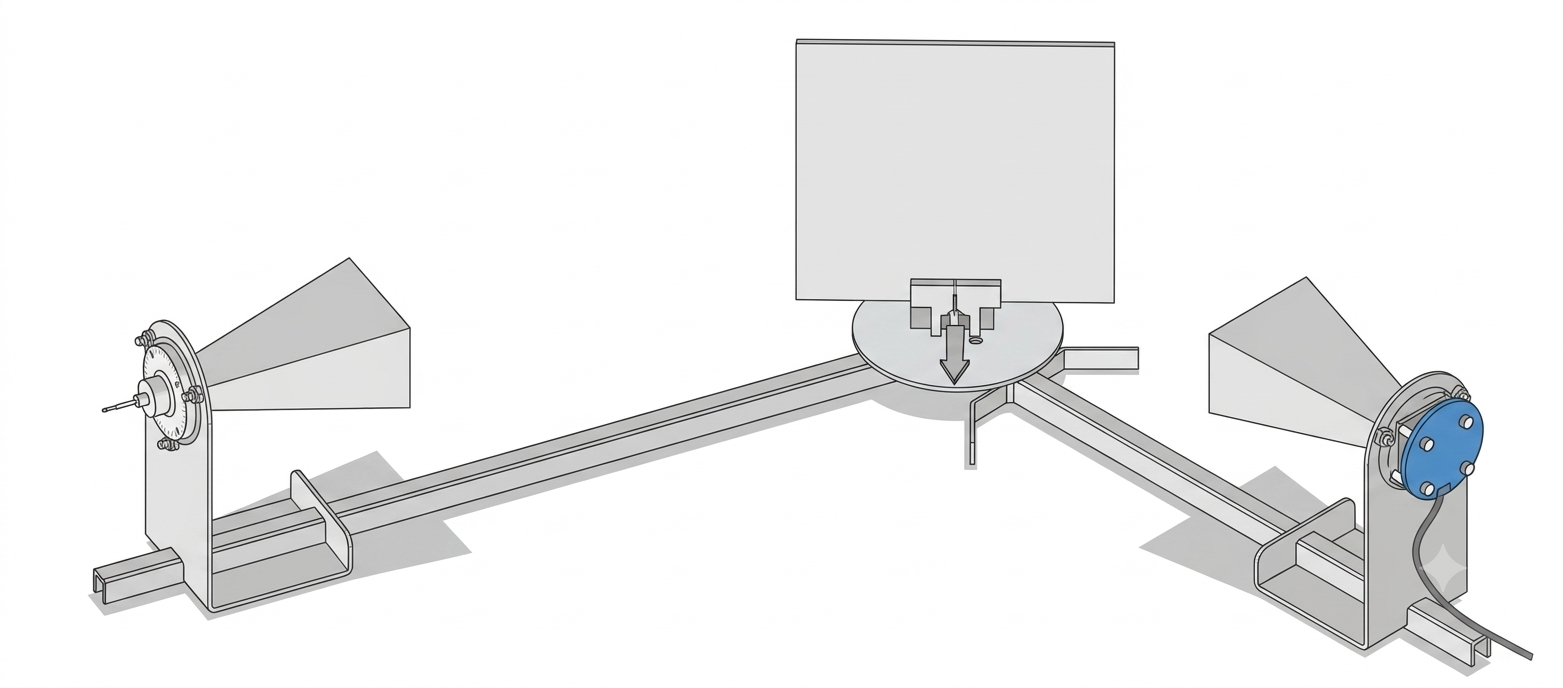
\includegraphics[width=0.5\textwidth]{Fig4}
		\captionof{figure}{\textit{Experimental setup for reflection of microwaves}}
	\end{center}
	\begin{enumerate}[leftmargin=1.5em]
		\item Set up the transmitter and receiver so that the angle of incidence can be read off.
		\item Line up the reflector plate at an angle of approximately $30^\circ$ with the help of the pointer for the rails, which points in the direction of the normal (a line perpendicular to the mirror's surface), as shown in Fig. 4.
		\item Change the angle of the long rail until maximum reception is attained. Measure the angles of incidence and reflection from the normal (arrow) and draw a conclusion.
		\item Repeat the procedure with other angles of the reflector, namely $40^\circ$, $50^\circ$, and $60^\circ$.
	\end{enumerate}
	
	\subsection*{2.5. Refraction of microwaves}
	\begin{center}
		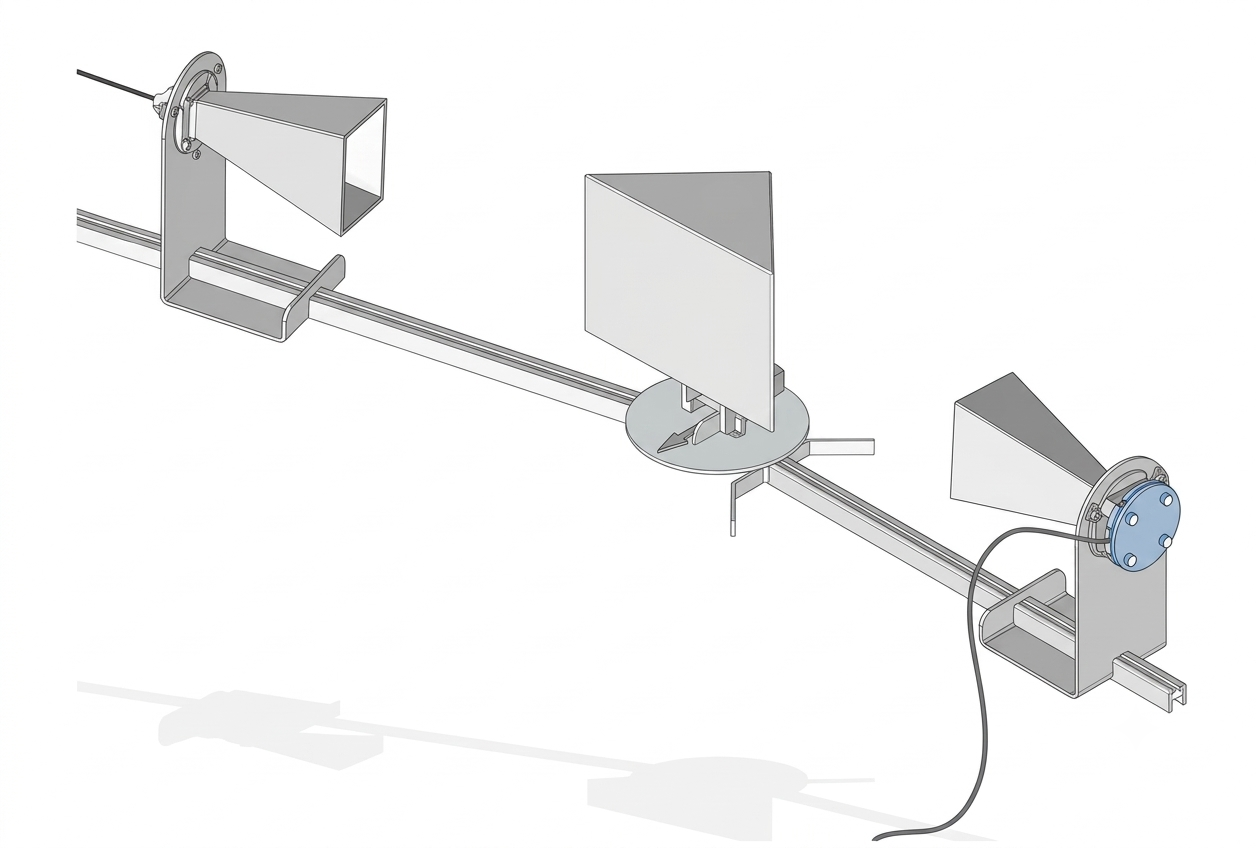
\includegraphics[width=0.5\textwidth]{Fig5}
		\captionof{figure}{\textit{Experimental setup for refraction of microwaves}}
	\end{center}
	\begin{enumerate}[leftmargin=1.5em]
		\item Set up the accessories including the transmitter, receiver, and prism on its stand facing away from the arrow, as shown in Fig. 5.
		\item Turn the long rail until maximum reception is attained. Observe and draw a conclusion on the reception of the signal.
	\end{enumerate}
	
	\subsection*{2.6. Diffraction of microwaves}
	\begin{center}
		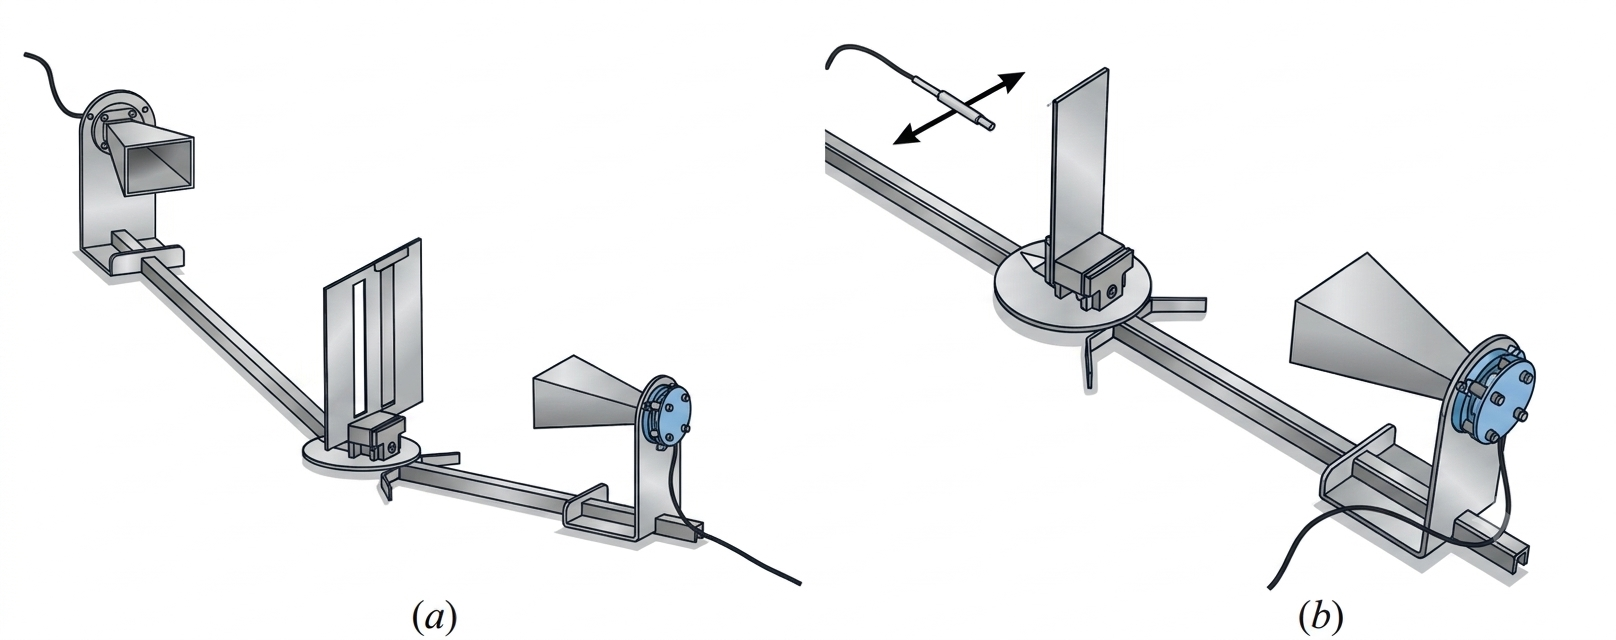
\includegraphics[width=0.8\textwidth]{Fig6}
		\captionof{figure}{\textit{Experimental setup for diffraction of microwaves}}
	\end{center}
	\begin{enumerate}[leftmargin=1.5em]
		\item Set up the accessories including the transmitter and receiver directly facing each other about $80\text{ cm}$ apart, as shown in Fig. 6a. Turn the receiver around on its rail so that it is out of the bundled microwave beam and the signal is clearly weakened.
		\item Place the single-slit plate (with the slit width smaller than the wavelength) vertically aligned about $20\text{ cm}$ in front of the transmitter so that the receiver once more detects a signal.
		\item Observe and draw a conclusion on the reception of the signal showing that microwaves are diffracted by the slit and wavelets can be detected in the shadow of the aperture.
		\item Clamp the cover plate in the holder on the hinge plate and set up the transmitter about $20\text{ cm}$ in front of the plate, as shown in Fig. 6b.
		\item Move the probe in a horizontal plane behind the plate. Observe and record the corresponding signal on the multimeter. Draw conclusions from the experimental results, especially when the probe is in the shadow of the plate.
	\end{enumerate}
	
	\subsection*{2.7. Interference of microwaves}
	\begin{center}
		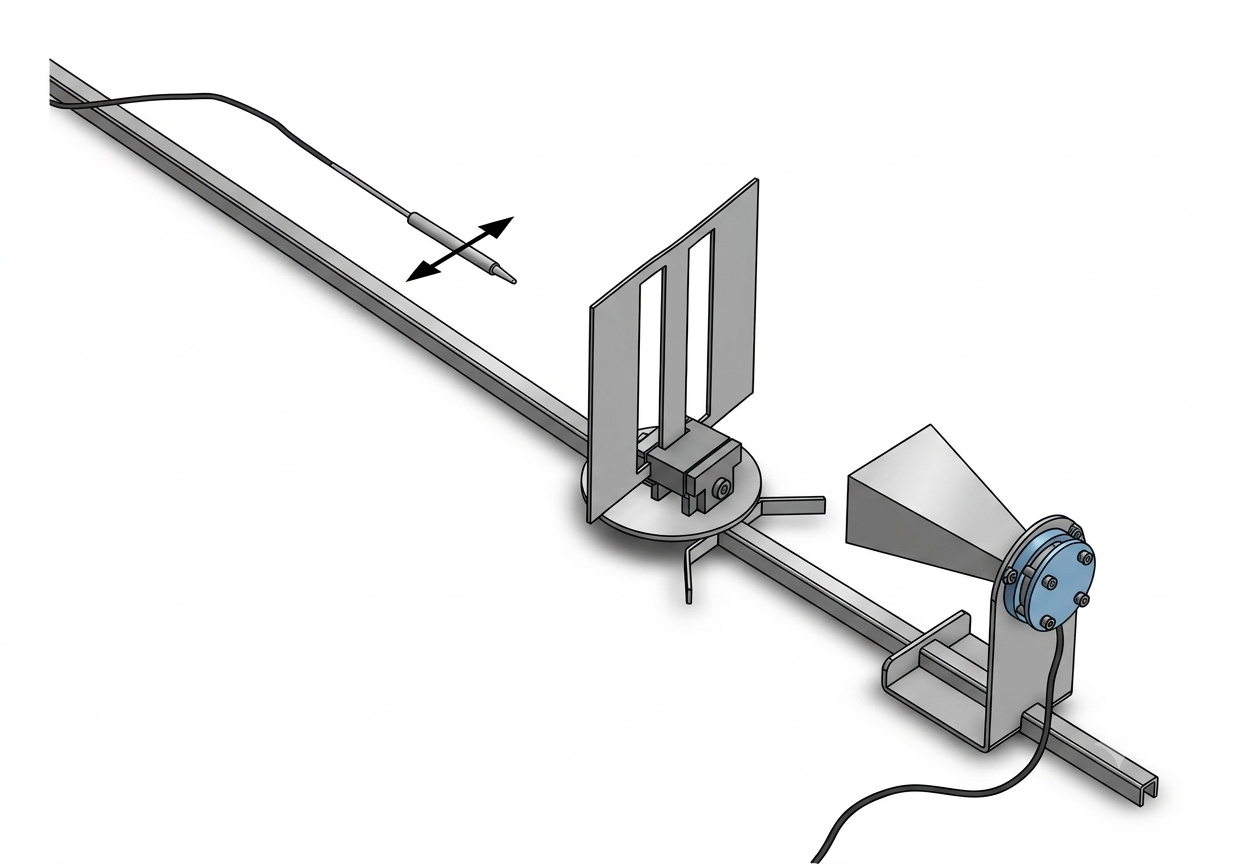
\includegraphics[width=0.5\textwidth]{Fig7}
		\captionof{figure}{\textit{Experimental setup for interference of microwaves}}
	\end{center}
	\begin{enumerate}[leftmargin=1.5em]
		\item Clamp the plate with the double slit centrally in the holder on the plate over the hinge. Position the transmitter about $12\text{ cm}$ in front of the plate. Place the receiver probe, which is connected to a multimeter, about $6\text{ cm}$ behind the double-slit plate, as shown in Fig. 7.
		\item Move the receiver probe parallel to the double-slit plate, as illustrated in Fig. 7. Observe and record the number of interference maxima corresponding to the signal on the digital multimeter. Draw conclusions from the experimental results.
	\end{enumerate}
	
	\subsection*{2.8. Polarization of microwaves}
	\begin{center}
		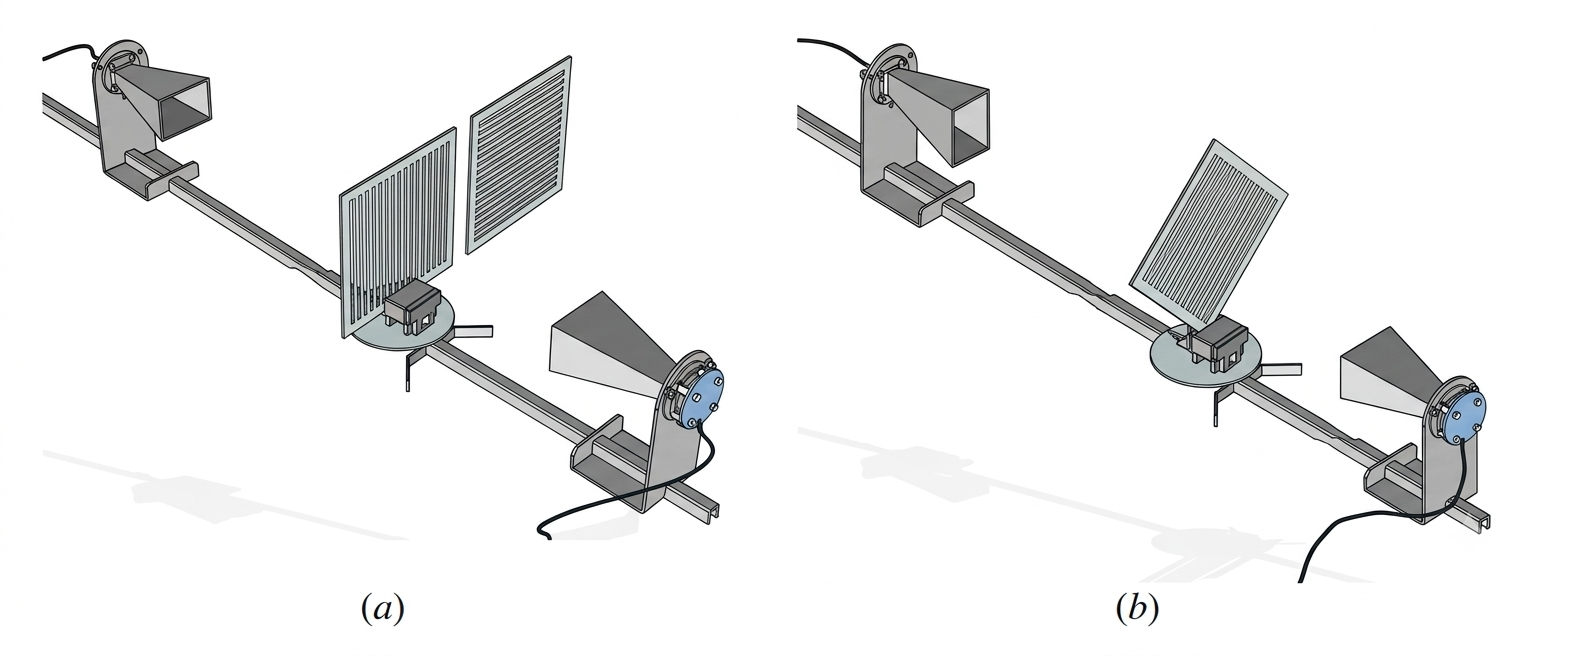
\includegraphics[width=0.8\textwidth]{Fig8}
		\captionof{figure}{\textit{Experimental setup for polarization of microwaves}}
	\end{center}
	\begin{enumerate}[leftmargin=1.5em]
		\item Set up the polarization grating in the screen holder.
		\item Check the reception when the polarization grating is aligned horizontally and vertically, as illustrated in Fig. 8a. Draw conclusions about the receiver's signal and provide explanations for the experimental results in both cases.
		\item Check the reception when the polarization grating is introduced into the beam and tilted by $45^\circ$, as shown in Fig. 8b. Draw conclusions about the receiver's signal and explain the experimental results.
	\end{enumerate}
	
	\subsection*{2.9. Wavelength of standing waves}
	\begin{center}
		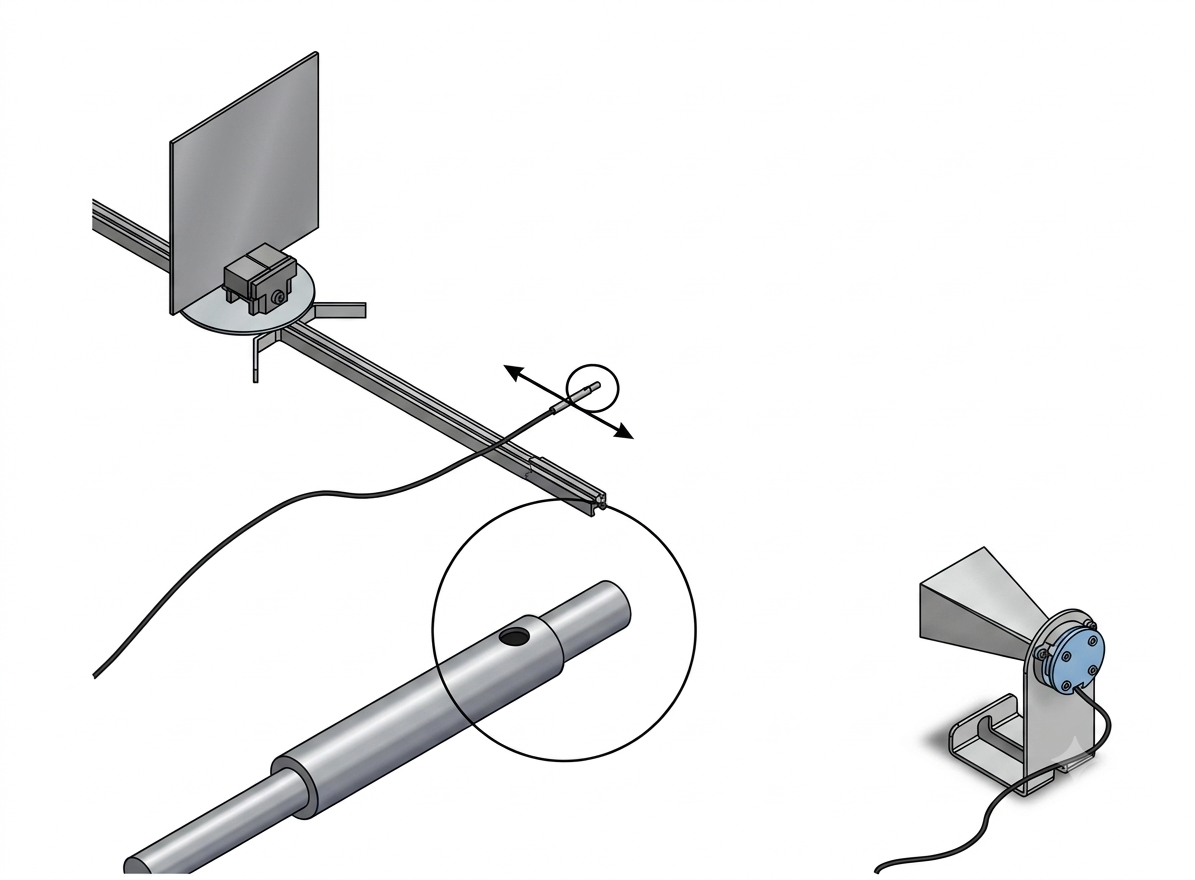
\includegraphics[width=0.5\textwidth]{Fig9}
		\captionof{figure}{\textit{Experimental setup for measuring the wavelength of standing waves}}
	\end{center}
	Set up the transmitter and reflector plate facing each other about $50\text{ cm}$ apart (in this case, the angle of incidence is $0^\circ$), as shown in Fig. 11. The transmitted and reflected waves are superimposed, resulting in a standing wave such that the wavelength corresponds to twice the distance between two adjacent minima (or maxima), i.e., $\lambda = 2d$.
	\begin{enumerate}[leftmargin=1.5em]
		\item Roughly investigate the interference maxima and minima of the transmitted and reflected waves by moving the microwave probe on the surface of and along the long bench, as illustrated in Fig. 9.
		\item Place the probe at the position corresponding to an interference maximum (or minimum) by observing the display on the voltmeter, and record that position as $x_1$. Afterward, continue moving the probe to the adjacent position of an interference maximum (or minimum) and record that position as $x_2$. Consequently, determine the distance between these two positions as $d = |x_2 - x_1|$.
		\item Repeat Step 2 two more times and record the measurement results in a data table with 4 columns: Trial, $x_1$, $x_2$, and $d$, respectively.
	\end{enumerate}
	
	\section*{3. EXPERIMENTAL RESULTS}
	
	\subsection*{3.1. Investigation of straight-line propagation of microwaves}
	\noindent
	When the receiver is aligned with the rail (the transmitter and the receiver are facing each other), the volt-meter shows the maximum value.
	
	\noindent
	When the receiver moves far from the rail (in a plane perpendicular to the rail), the value showed on the volt-meter decreases.
	
	\noindent
	Hence, microwaves propagate best in a straight line.
	\subsection*{3.2. Investigation of penetration of microwaves}
	\noindent
	When a dry absorption plate is put between the transmitter and the receiver, the value showed on the volt-meter slightly decreases.
	
	\noindent
	We can conclude that microwaves can penetrate through the dry absorption plate, but not all of the microwaves will penetrate through the dry absorption plate. Instead, a part of them will be absorbed by the absorption plate.
	
	\subsection*{3.3. Investigation of screening and absorption of microwaves}
	\noindent
	When a reflection plate is put between the transmitter and the receiver, the volt-meter shows a value close to 0 (0.01). It implies that the reflection plate screens the microwaves by reflecting them, preventing them from passing through.
	
	\subsection*{3.4. Investigation of reflection of microwaves}
	\noindent
	After trying multiple reflector angles, we yield a data table recording the incidence angles making the volt-meter show maximum value.
	\begin{table}[H]
		\centering
		\begin{tabular}{|>{\centering\arraybackslash}m{1.5cm}|>{\centering\arraybackslash}m{4.5cm}|>{\centering\arraybackslash}m{4.5cm}|}
			\hline
			\textbf{Trial} & \textbf{Reflector angle$\left(^\circ\right)$} & \textbf{Incidence angle$\left(^\circ\right)$} \rule[-0.2cm]{0pt}{0.6cm} \\
			\hline
			1 & 30 & 30 \rule[-0.25cm]{0pt}{0.7cm} \\
			\hline
			2 & 40 & 40 \rule[-0.25cm]{0pt}{0.7cm} \\
			\hline
			3 & 50 & 50 \rule[-0.25cm]{0pt}{0.7cm} \\
			\hline
			4 & 60 & 60 \rule[-0.25cm]{0pt}{0.7cm} \\
			\hline
		\end{tabular}
	\end{table}
	\noindent
	Hence, we can conclude that microwaves reflects best when the perpendicular bisector of the reflection plate is the  bisector  of  an  angle  created  by  the  transmitter  and  receiver; and when the microwaves reflect, the angle of incidence equals the angle of reflection.
	
	
	\subsection*{3.5. Investigation of refraction of microwaves}
	\noindent
	When the angle created by 2 rails is $150^\circ$, the volt-meter shows the maximum value. Turning the receiver to a different angle makes the value showed on the volt-meter decreases.
	
	\noindent
	We can conclude that: When microwaves pass through the paraffin prism, they undergo refraction (bending). The angle of $150^\circ$ corresponds to the angle of deviation where the refracted beam has the highest intensity.
	
	\subsection*{3.6. Investigation of diffraction of microwaves}
	\noindent
	When the single slit plate is put in the rail, the value showed on the volt-meter increases.
	
	\noindent
	When the cover plate is between the probe and the transmitter, the value showed on the volt-meter is approximate 0 in the shadow. When the probe is moved on the horizontal plane behind the plate, the value slightly increases.
	
	\noindent
	All evidences show that microwaves diffract. They curve around the edges of an obstacle (like a cover plate) and spread into the shadow region after traveling through a single-slit opening.
	
	\subsection*{3.7. Investigation of interference of microwaves}
	\noindent
	When the probe is moved parallel to the plate, the value showed on the volt-meter is oscillating. The number of interference maxima is 3. It implies that microwaves have the property of interference.
	
	\subsection*{3.8. Investigation of polarization of microwaves}
	\noindent
	When the grating is aligned horizontally, the value showed on the volt-meter almost unchanges.
	
	\noindent
	When the grating is aligned vertically, the value showed on the volt-meter is approximate to $0$.
	
	\noindent
	When the grating is aligned at $45^\circ$, the value showed on the volt-meter is higher than that in vertical case, but lower than that in horizontal case.
	
	\noindent
	These results demonstrate that microwaves are transverse, linearly polarized waves (polarized vertically in this setup), and their transmission through a polarizing grating depends on the angle between the grating bars and the wave's plane of polarization.
	
	
	\subsection*{3.9. Wavelength and Frequency of Microwaves}
	\subsubsection*{3.9.1. Data Table}
	
	\begin{table}[H]
		\centering
		\caption{Measurement of standing wave positions}
		\begin{tabular}{|>{\centering\arraybackslash}m{1.5cm}|>{\centering\arraybackslash}m{4cm}|>{\centering\arraybackslash}m{4cm}|>{\centering\arraybackslash}m{4cm}|}
			\hline
			\textbf{Trial} & \textbf{$x_1$ (mm)} & \textbf{$x_2$ (mm)} & \textbf{$d$ (mm)} \rule[-0.2cm]{0pt}{0.6cm} \\
			\hline
			1 & 160 & 175 & 15 \rule[-0.25cm]{0pt}{0.7cm} \\
			\hline
			2 & 175 & 190 & 15 \rule[-0.25cm]{0pt}{0.7cm} \\
			\hline
			3 & 190 & 206 & 16 \rule[-0.25cm]{0pt}{0.7cm} \\
			\hline
		\end{tabular}
	\end{table}
	
	\subsubsection*{3.9.2. Data Processing}
	
	\noindent
	The mean value of $d$ is
	\begin{center}
		\fbox{%
			\begin{minipage}{0.8\textwidth}
				\vspace{-0.4cm}
				\centering
				\begin{displaymath}
					\overline{d} = \frac{d_1 + d_2 + d_3}{3} = \dfrac{46}{3} \left(\text{mm}\right)
				\end{displaymath}
			\end{minipage}%
		}
	\end{center}
	
	\noindent
	The standard deviation of a single measurement is
	\begin{center}
		\fbox{%
			\begin{minipage}{0.8\textwidth}
				\vspace{-0.4cm}
				\centering
				\begin{displaymath}
					\text{sd}_d = \sqrt{\frac{\left(d_1 - \overline{d}\right)^2 + \left(d_2 - \overline{d}\right)^2 + \left(d_3 - \overline{d}\right)^2}{3}} = \dfrac{\sqrt{2}}{3} \left(\text{mm}\right)
				\end{displaymath}
			\end{minipage}%
		}
	\end{center}
	
	\noindent
	And the standard deviation of the mean is
	\begin{center}
		\fbox{%
			\begin{minipage}{0.8\textwidth}
				\vspace{-0.4cm}
				\centering
				\begin{displaymath}
					\text{SD}_d = \frac{\text{sd}_d}{\sqrt{3}} = \dfrac{\sqrt{6}}{9} \left(\text{mm}\right)
				\end{displaymath}
			\end{minipage}%
		}
	\end{center}
	
	\noindent
	Using $\lambda = 2d$, the mean wavelength and its uncertainty are
	\begin{center}
		\fbox{%
			\begin{minipage}{0.8\textwidth}
				\vspace{-0.4cm}
				\centering
				\begin{displaymath}
					\begin{aligned}
						&\overline{\lambda} = 2\overline{d} = \dfrac{92}{3} \left(\text{mm}\right) \approx 30.667  \left(\text{mm}\right) \\
						&\Delta \lambda = 2\,\text{SD}_d = \dfrac{2\sqrt{6}}{9} \left(\text{mm}\right) \approx 0.544  \left(\text{mm}\right)
					\end{aligned}
				\end{displaymath}
			\end{minipage}%
		}
	\end{center}
	
	\noindent
	Therefore, our result for $\lambda$ appears as
	\begin{center}
		\fbox{%
			\begin{minipage}{0.8\textwidth}
				\vspace{-0.4cm}
				\centering
				\begin{displaymath}
					\lambda = \overline{\lambda} \pm \Delta \lambda = 30.667 \pm 0.544 \left(\text{mm}\right)
				\end{displaymath}
			\end{minipage}%
		}
	\end{center}
	
	\noindent
	Using $c = \lambda f$ with $c = 3 \times 10^8\text{ m/s}$, the mean frequency and its uncertainty are
	\begin{center}
		\fbox{%
			\begin{minipage}{0.8\textwidth}
				\vspace{-0.4cm}
				\centering
				\begin{displaymath}
					\begin{aligned}
						&\overline{f} = \frac{c}{\overline{\lambda}} = \dfrac{3 \times 10^8}{\dfrac{92}{3} \times 10^{-3}} = \dfrac{900}{92} \times 10^9 \approx 9.783 \times 10^9 \left(\text{Hz}\right) \\
						&\Delta f = \overline{f} \cdot \frac{\Delta \lambda}{\overline{\lambda}} = \dfrac{900}{92} \times 10^9 \times \dfrac{\dfrac{2\sqrt{6}}{9} \times 10^{-3}}{\dfrac{92}{3} \times 10^{-3}} \approx 0.174 \times 10^9 \left(\text{Hz}\right)
					\end{aligned}
				\end{displaymath}
			\end{minipage}%
		}
	\end{center}
	
	\noindent
	Therefore, our result for $f$ appears as
	\begin{center}
		\fbox{%
			\begin{minipage}{0.8\textwidth}
				\vspace{-0.4cm}
				\centering
				\begin{displaymath}
					f = \overline{f} \pm \Delta f = \left(9.783 \pm 0.174\right) \times 10^9 \left(\text{Hz}\right)
				\end{displaymath}
			\end{minipage}%
		}
	\end{center}
	
\end{document}
